%%%%%%%%%%%%%%%%%%%%%%%%%%%%%%%%%%%%%%%%%%%%%%%%%%%%%%%%%%%%%%%%%%%%%%%%%%
%% Review Volume (last updated on 2014/03/05)                           %%
%% Trim Size: 9.61in x 6.69in                                           %%
%% Text Area: 8in (include runningheads) x 5in                          %%
%% Main Text: 10 on 13pt                                                %%
%% For support: Yolande Koh, <ykoh@wspc.com.sg>                         %%
%%              D. Rajesh Babu, <rajesh@wspc.com.sg>                    %%
%%%%%%%%%%%%%%%%%%%%%%%%%%%%%%%%%%%%%%%%%%%%%%%%%%%%%%%%%%%%%%%%%%%%%%%%%%
%%
%\documentclass[wsdraft]{ws-rv961x669} % to draw border line around text area
\documentclass{ws-rv961x669}
\usepackage{ws-rv-van}     % numbered citation/references (default)
\usepackage{ws-rv-thm}     % comment this line when `amsthm / theorem / ntheorem` package is used
\usepackage{subfigure}     % required only when side-by-side / subfigures are used
\usepackage{caption}
\usepackage{threeparttable}
%\usepackage{ws-index}     % required only when multiple indexes are used
\makeindex
%\newindex{aindx}{adx}{and}{Author Index}       % author index
%\renewindex{default}{idx}{ind}{Subject Index}  % subject index

\begin{document}

\chapter[Spectrometers]{Spectrometers}\label{spec_chap}

\author[D. Price and J. Hickish]{Danny C. Price and J. Hickish}

\address{Campbell Hall 339, UC Berkeley\\
Address goes here, \\
dancpr@berkeley.edu}

\begin{abstract}
This review gives an introduction to spectrometers and discusses their use within radio astronomy. While a variety of technologies are introduced, particular emphasis is given to digital systems
%, with details of current-generation implementations given as examples. 
Three different types of digital spectrometers are discussed: autocorrelation spectrometers, Fourier transform spectrometers, and polyphase filterbank spectrometers.  Given their growing ubiquity and significant advantages, polyphase filterbanks are detailed at length. The relative advantages and disadvantages of different spectrometer technologies are compared and contrasted, and implementation considerations are presented.

\end{abstract}

%\markright{Customized Running Head for Odd Page} % default is Chapter Title.

\body

\section{Introduction}\label{sec:intro}

A \emph{spectrometer} is a device used to record and measure the spectral content of signals, such as radio waves received from astronomical sources. Specifically, a spectrometer measures the power spectral density (PSD, measured in units of $\rm{WHz}^{-1}$) of a signal. Analysis of spectral content can reveal details of radio sources, as well as properties of the intervening medium. For example, spectral line emission from simple molecules such as neutral hydrogen gives rise to narrowband radio signals (Fig.~1), while continuum emission from active galactic nuclei gives rise to wideband signals.


There are two main ways in which the PSD --- commonly known as \emph{power spectrum} --- of a signal may be computed. The power spectrum, $S_{xx}$, of a waveform and its autocorrelation function,  $r_{xx}$, are related by the Wiener-Khinchin theorem. This theorem states that the relationship between a stationary (mean and variance do not change over time), ergodic (well-behaved over time) signal $x(t)$, its PSD, and its autocorrelation is given by
\begin{equation}
S_{xx}(\nu)=\int_{-\infty}^{\infty}r_{xx}(\tau)e^{-2\pi i\nu\tau}d\tau.
\label{eq:psd}
\end{equation}
where $\nu$ represents frequency, and $\tau$ represents a time delay or `lag'. The autocorrelation function is
\begin{equation}
r_{xx}(\tau)=\left\langle x(t)x(t-\tau)\right\rangle,
\end{equation}
where angled brackets refer to averaging over time. 

\begin{figure}[t]
 \centering
 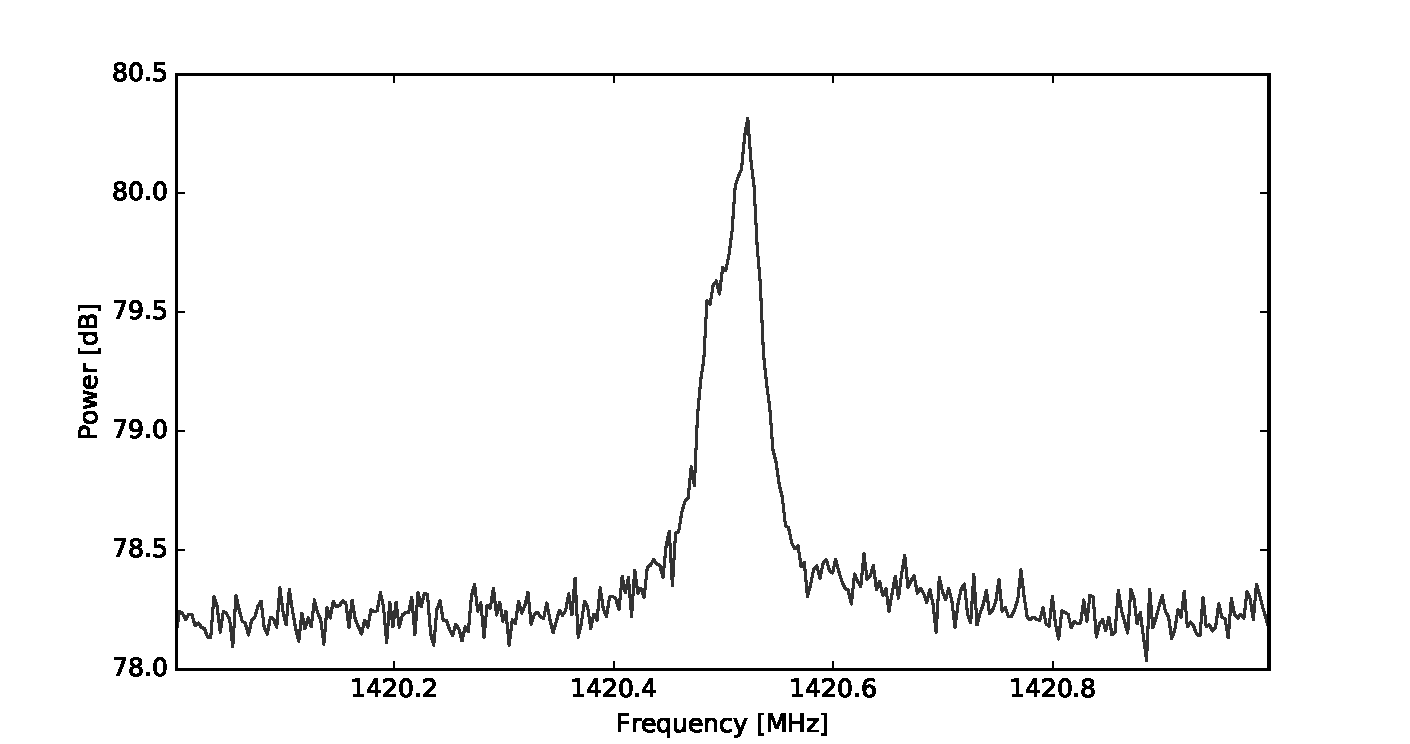
\includegraphics[width=\textwidth]{./figures/hydrogen.pdf}
 % analog-autocorr-crop.pdf: 0x0 pixel, 0dpi, nanxnan cm, bb=
 \label{fig:hydrogen}
 \caption{A galactic hydrogen 21-cm line emission profile, as measured using a digital spectrometer system on the Robert C. Byrd Greenbank Telescope in West Virginia.}
\end{figure}

Equation~\ref{eq:psd} shows that that the autocorrelation function is related to the PSD by a Fourier transform. In the discrete case, the relationship becomes
\begin{equation}
S_{xx}(k)=\sum_{k=-\infty}^{\infty}\left\langle x(n)x(n-k)\right\rangle e^{-2\pi ik\tau},\label{eq:discrete-wiener}
\end{equation}
which may be recognized as a discrete convolution. It follows from the convolution theorem that 
\begin{equation}
S_{xx}(k)=\left\langle \left|X(k)\right|^{2}\right\rangle ,\label{eq:discrete-pow}
\end{equation}
where $X(k)$ denotes the Discrete Fourier Transform (DFT) of $x(t)$:
\begin{equation}
X(k)=\sum_{n=0}^{N-1}x(n)e^{-2\pi ink/N}\label{eq:dft1}
\end{equation}

There are therefore two distinct classes of spectrometers: ones that approximate $S_{xx}(k)$ by firstly forming the autocorrelation, then taking a Fourier transform a~la Eq.~\ref{eq:discrete-wiener}, and those that first convert into the frequency domain to form $X(k)$ before evaulating Eq.~\ref{eq:discrete-pow}. These two routes are shown diagramatically in Fig.~\ref{fig:wiener}. We will refer to these as autocorrelation spectrometers (ACS, Sec.~\ref{sub:acs}), and Fourier transform filterbanks (FTF, Sec.~\ref{sub:ftf}), respectively. Polyphase filterbank spectrometers (PFB, Sec.~\ref{sub:pfb}) can be thought of as an  FTF with enhanced filter response. Note that because the DFT is an \emph{approximation} to the continuous Fourier Transform, ACS and FTF systems have different characteristics. 

% FIGURE
\begin{figure}[t]
 \centering
 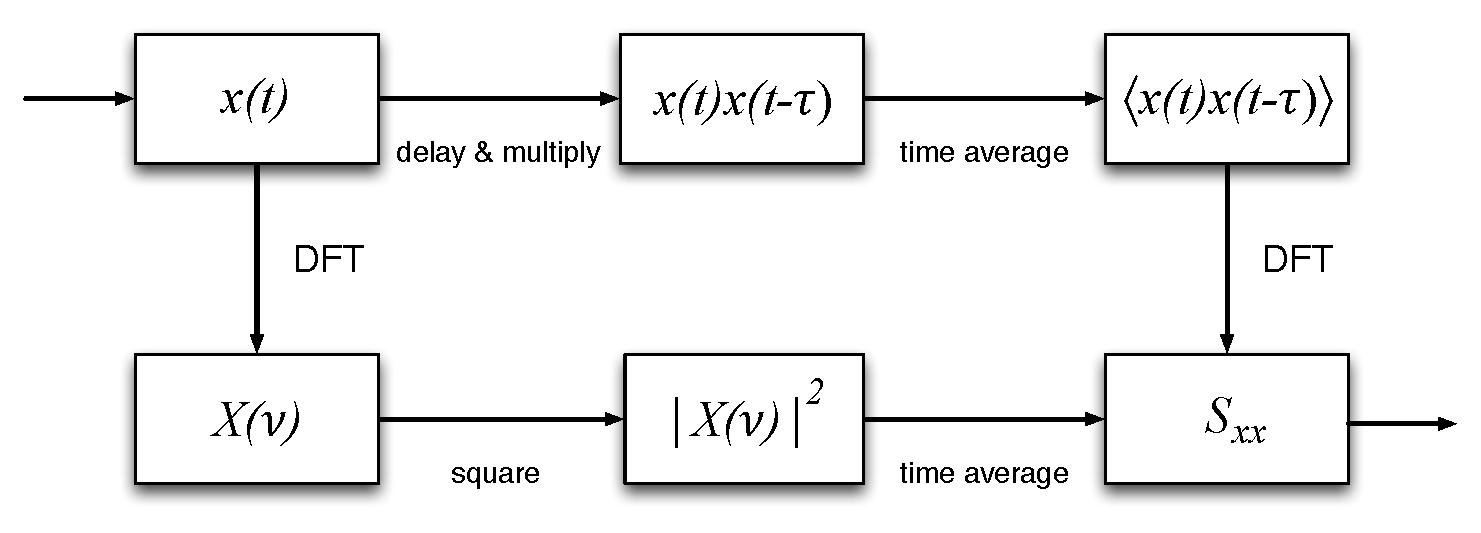
\includegraphics[width=0.9\textwidth]{./figures/wiener}
 \caption{The two methods used to compute the PSD of a signal. The top path corresponds to an ACS system while the bottom corresponds to an FTF system. The two approaches are related by the Wiener-Khinchin theorem. \label{fig:wiener}  }
\end{figure}
% FIGURE

\subsection{Analysis and synthesis filterbanks}

It is important to note the relationship between spectrometers, filters, and filterbanks. A \emph{filterbank} is simply an array of band-pass filters, designed to split an input signal into multiple components, or similarly, to combine multiple components. These are referred to as \emph{analysis} and \emph{synthesis} filterbanks, respectively. When applied to streaming data, a DFT can be considered an analysis filterbank, and an inverse DFT to be a synthesis filterbank. From this viewpoint, a spectrometer is simply an analysis filterbank, where the output of each filter is squared and averaged.

%Analysis and synthesis filterbanks have many applications outside of astronomy, see \cite{} for further discussion.

\subsection{Polarimetry}

Polarization is a key measurement within radio astronomy.\citet{BookTinbergenPolarim}  Although most astrophysical radio emission is inherently unpolarized, a number of radio sources --- such as pulsars and masers --- do emit polarized radiation, and effects such as Faraday rotation by a galactic magnetic fields can yield polarized signals. A spectrometer that also measures polarization is known as a \emph{polarimeter} (or spectropolarimeter).

\subsubsection{Stokes parameters}

The Stokes parameters are a set of four quantities which fully describe the polarization state of an electromagnetic wave; this is what a polarimeter must measure. The four Stokes parameters, $I$, $Q$, $U$ and $V$, are related to the amplitudes of perpendicular components of the electric field:
\begin{eqnarray}
E_{x} & = & e_{x}(t)cos(\omega t+\delta_{x})\\
E_{y} & = & e_{y}(t)cos(\omega t+\delta_{y})
\end{eqnarray}
by time averages of the electric field parameters:
\begin{eqnarray}
I & = & \left\langle E_{x}E_{x}^{*}+E_{y}E_{y}^{*}\right\rangle \\
Q & = & \left\langle E_{x}E_{x}^{*}-E_{y}E_{y}^{*}\right\rangle \\
U & = & \left\langle E_{x}E_{y}^{*}+E_{y}E_{x}^{*}\right\rangle \\
V & = & i\left\langle E_{x}E_{y}^{*}-E_{y}E_{x}^{*}\right\rangle 
\end{eqnarray}
where $*$ represents conjugation. The parameter $I$ is a measure of the total power in the wave, $Q$ and $U$ represent the linearly polarised components, and $V$ represents the circularly polarised component. The Stokes parameters have the dimensions of flux density, and they combine additively for independent waves.

\subsubsection{Measuring polarization products}

In order to compute polarization products, a spectrometer must be presented with two voltage signals, $x(t)$ and $y(t)$, from a dual-polarization feed (i.e. a set of orthogonal antennas). With analogy to Eq.~\ref{eq:discrete-pow}, we may form 
\begin{eqnarray}
S_{xx}(k) & =  \langle X(k)X^*(k)\rangle  & = \langle |X(k)|^2\rangle \label{eq:sxx1} \\
S_{yy}(k) & =  \langle Y(k)Y^*(k)\rangle  & = \langle |Y(k)|^2\rangle \\
S_{xy}(k) & =  \langle X(k)Y^*(k)\rangle  & \\
S_{yx}(k) & =  \langle Y(k)X^*(k)\rangle  & \label{eq:sxx4}
\end{eqnarray}
where in addition to measuring the PSD of $x(t)$ and $y(t)$, we also compute their cross correlations.  Note that while $S_{xx}$ and $S_{yy}$ are real valued, $S_{xy}$ and $S_{yx}$ are complex valued.

The four terms $\langle E_x E_x^*\rangle$, $\langle E_y E_y^* \rangle$, $\langle E_x E_y^* \rangle$, and $\langle E_y E_x^* \rangle$ are linearly related (by calibration factors) to the quantities in Eq.~\ref{eq:sxx1}-\ref{eq:sxx4} above. Combining these therefore allows for Stokes $I$, $Q$, $U$ and $V$ to be determined.

In order to focus on the fundamental characteristics of spectrometers, the remainder of this chapter details single-polarization systems that compute only $S_{xx}$. Nevertheless, the techniques and characterization approaches are broadly applicable to polarimetry systems.

%\subsection{Radiometry and signal to noise}

%Noise is inherent in any radio-frequency instrument. The system temperature, $T_{\rm{sys}}$, is a measure of the total noise of a telescope, including the noise contribution from the sky and antenna. To mitigate the effect of noise, one can take multiple measurements over bandwidth and time. The time it takes to reach a target root-mean-square noise temperature is then given by the ideal radiometer equation: 
%\begin{equation}
%\sigma_{T}=\frac{T_{sys}}{\sqrt{\Delta\nu t}},\label{eq:radiometer-eqn}
%\end{equation}
%where $t$ is integration time. The smallest detectable signal $T_{S}$ is given by $T_{S}=m\sigma_T$, where $m$ is a threshold value, generally greater than or equal to 3. 

%Spectrometers can increase the signal-to-noise ratio (SNR) of a radio telescope through both integration and channelization. Integration increases the SNR because signal increases linearly with integration whereas noise increases as the square root with integration. Thus, integrating longer by a factor of N will increase SNR by a factor of $\sqrt{N}$, as shown in Eq.~\ref{eq:radiometer-eqn}.

%Channelization reduces the signal to noise of narrowband signals due to the fact that the noise power will be divided equally across spectral channels, while the narrowband signal is confined to a comparatively fewer channels. For sinusoidal signals, channelizing to N channels will reduce the per-channel noise power by a factor of N, thereby increasing the per-channel SNR by a factor of N.

\subsection{Performance characteristics}

\begin{figure}
 \centering
 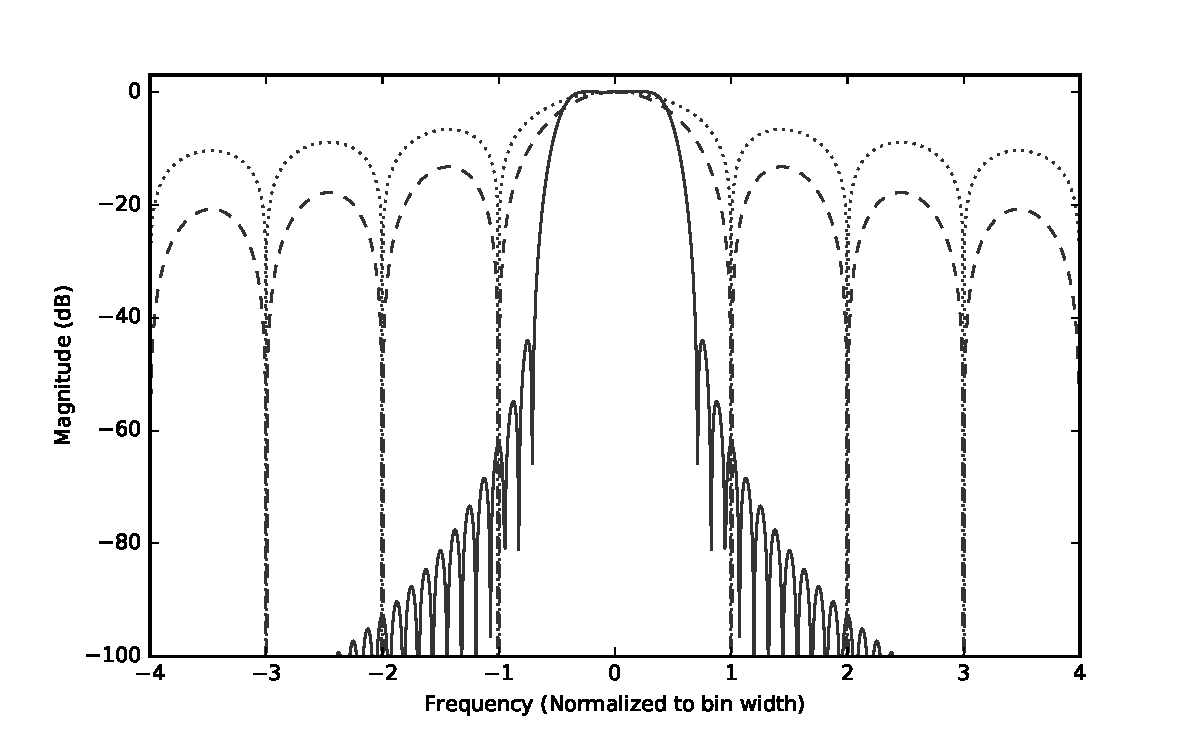
\includegraphics[width=\textwidth]{./figures/fb_comparison}
 \label{fig:pfb_response}
 \caption{Comparison of the filter response of an ACS (dotted line), FTF (dashed line) and an 8-tap, Hann-windowed PFB (solid line).\label{fig:leakage}}
\end{figure}

%There are several important characteristics to consider when comparing spectrometer implementations. 

\subsubsection{Spectral leakage}
Spectrometers operate over a finite bandwidth $B$, over which $N$ channels with bandwidth $\Delta\nu = B/N$ are computed. With digital filters, it is possible for each channel to be evenly spaced and to have identical filter shapes. 

Ideally, each channel would have unitary response over $\nu_c \pm \frac{\Delta\nu}{2}$, where $\nu_c$ is the center frequency, with zero response outside this passband. In practice, this cannot be achieved; each channel has a non-zero response over all frequencies.  As such, a signal will `leak' between neighboring channels, known as spectral leakage.

Fig.~\ref{fig:leakage} compares the normalized filter response for ACS, FTF and PFB implementations. In the presence of strong narrowband signals, such as radio interference (RFI), spectral leakage is a major concern.

\subsubsection{Scalloping loss} 

A related concern is that the channel's non-ideal shape will cause narrowband signals at channel edges to be attenuated, an effect known as scalloping loss (Fig.~\ref{fig:scalloping}). Spectrometers are often designed such that neighboring channels overlap at their full-width at half-maximum points (FWHM), in which case the signal will be spread evenly over both channels. Wideband signals are not affected by scalloping. 

\begin{figure}
 \centering
 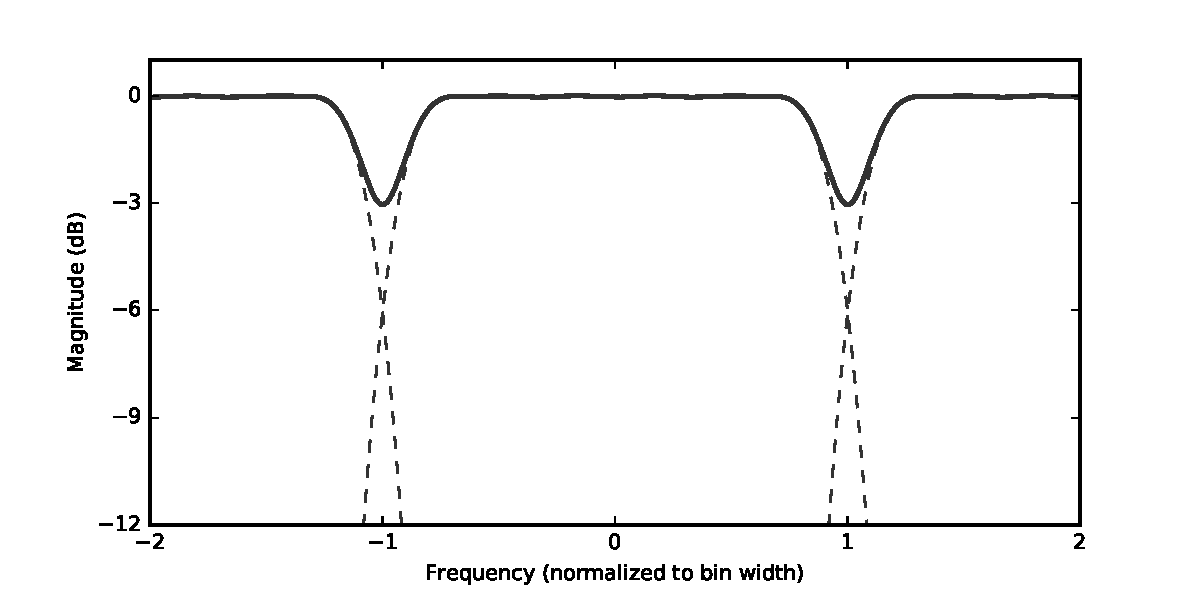
\includegraphics[width=\textwidth]{./figures/pfb_scalloping}
 \caption{Example of scalloping loss between spectrometer channels. The dashed lines show the response of individual channels, while the black line shows the overall response.\label{fig:scalloping}}
\end{figure}

\subsubsection{Time resolution} 

Time resolution refers to the minimum integration time, $t_{\rm{min}}$, over which a spectrometer computes the time average. Detection of transient phenomena, such as fast radio bursts\cite{Lorimer2007} and pulsars, require $t_{\rm{min}}$ to be as short as a nanosecond; integration lengths of several seconds are common when observing faint sources. The minimum and maximum averaging times are generally enforced by hardware limitations.

\subsubsection{Dynamic range}
Dynamic range refers to the span of input powers over which a spectrometer can operate nominally. The presence of RFI and the input bandwidth are the main drivers for dynamic range; see Sec.~\ref{sub:dynamic-range}.

%PFB spectrometers offer less scalloping loss and spectral leakage than both ACS and FTF implementations. Nevertheless, ACS and FTF systems are still encountered within radio astronomy. Further comparison of architectures is given in Sec.~\ref{sub:comparison}.



\section{Digital systems}

Digital signal processing (DSP) techniques are well-suited to applications such as filtering and forming filterbanks; as such, a majority of current-day spectrometers are based on digital technology. A basic understanding of DSP is required to fully understand digital spectrometers; there are several excellent introductory DSP texts available \cite{Lyons:2000uy, BookSmithFFT}. 

In the diagrams and equations that follow, the symbol $\otimes$ denotes multiplication of time samples; $\oplus$ denotes addition. The symbol $z^{-n}$ is used to denote a time delay of \emph{n} units, due to the relationship between time delay in a digital stream and the z-transform. 

\subsection{Digital sampling}

Digital sampling, or digitization, is the process of converting an analog signal to a digital one; devices known as analog to digital converters (ADCs) do this conversion. The two main characteristics of an ADC are its sample rate, $\nu_{\rm{s}}$, and the number of bits per sample, $n_{\rm{bits}}$.

\subsubsection{Nyquist sampling \label{sub:sampling}}

An ADC converts an analog voltage waveform into a series of numeric quantities called samples. The sample rate determines the amount of bandwidth that can be unambiguously processed by an ADC. The Nyquist Theorem --- one of the most fundamental theorems within signal processing --- states that a band-limited signal may be fully recovered when it is sampled at a rate that is twice the bandwidth, $\nu_{\rm{s}} = 2 B$. 
% the Nyquist rate is therefore dependent upon a given signal's bandwidth. 
%For example, a sample rate of 2 billion samples per second allows a band-limited signal with a bandwidth of 1~GHz to be digitized. 
Sampling at the  Nyquist rate is referred to as \emph{critical sampling}, under the Nyquist rate as \emph{undersampling}, and sampling over the Nyquist rate as \emph{oversampling}. Sample rates may be increased by a process known as \emph{upsampling} and decreased by \emph{downsampling}, by using sample rate conversion filters. We use the symbol $\downarrow D$ to denote downsampling by a factor \emph{D} and $\uparrow U$ for upsampling by a factor \emph{U}.

Undersampling a signal causes an effect known as \emph{aliasing} to occur, whereby different parts of a signal are indistinguishable from each other, resulting in information loss. Note that oversampling a signal does not increase the information content, but under certain circumstances is advantageous for reducing noise and/or distortion.


\subsubsection{Quadrature sampling}

\emph{Quadrature sampling}\cite{Lyons:2000uy} is the process of digitizing a band-limited signal and translating it to be centered about 0~Hz. A quadrature-sampled signal is complex valued, in contrast to real-valued Nyquist sampling. A quadrature-sampled signal has $\nu_{s} = B$; that is, each complex-valued sample is equivalent to two real-valued samples. Quadrature-sampled signals may have negative frequency components (i.e. below 0~Hz).

A Nyquist-sampled signal $x(t)$ centered at $\nu_0$ can be converted into a quadrature-sampled signal $x'(t)$ by multiplication with a complex phasor $e^{-2\pi i \nu_0 t}$:
\begin{equation}
	x'(t) = x(t) e^{-2 \pi i \nu_0 t},
\end{equation}
which is known as quadrature mixing.

The similarity between the phasor $e^{-2\pi i \nu_0 t}$ and that encountered in a DFT is noteworthy: each channel of a DFT can be seen quadrature mixing the input signal, applying a filter of width $B$, and then downsampling the signal to a rate $\nu_s=B$.

% \subsubsection{Compressed sampling}
% Compressed sampling [REF] is a recently discovered technique in which signals that exhibit sparsity can be reconstructed using fewer samples than the Nyquist rate. To date, compressive sampling has not been employed in radio astronomy spectrometers.

\subsubsection{Quantization efficiency \label{sub:quant}}

\begin{table}
	\caption{Quantization efficiencies $\eta_Q$ for Nyquist sampling with different bit depths $N_{\rm{bits}}$. Table modified from Thompson et. al.\citep{Thompson:2007p8886}.\label{tab:quant_eff}}
	\begin{center}
	\begin{tabular}{c c c c}
	\hline
	$N_{\rm{bits}}$ & $N_{\rm{levels}}$ & $\varepsilon$ & $\eta_Q$ \\
	\hline
	\hline
	2 & 4   & 0.995  & 0.88115 \\
	3 & 8   & 0.586  & 0.96256 \\
	4 & 16  & 0.335  & 0.98846 \\
	5 & 32  & 0.188  & 0.99651 \\
	6 & 64  & 0.104  & 0.99896 \\
	7 & 128 & 0.0573 & 0.99970 \\
	8 & 256 & 0.0312 & 0.99991 \\
	\hline
	\end{tabular}
	\end{center}
\end{table}

The earliest digital correlators \citep{Weinreb:1963p10042} used only two-level sampling (one bit), assigning a value of either +1 or -1. This scheme works remarkably well for weak, noise-dominated signals\footnote{That is, we assume that the probability distribution of the signal is close to Gaussian.}: for Nyquist-sampled signals, a signal-to-noise ratio of $2/\pi=0.637$ that of the unquantized signal is achievable [REF VAN VLECK 1966] (see Chapter 8 of TMS\citet{ThompsonMoranSwenson2004}). For 2-bit data, one can achieve 88\% quantization efficiency, which rises to 98\% for 4-bit data. Given these high values for low bit-widths, it is common to use bits sparingly within radio astronomy applications. A listing of quantization efficiencies\cite{Thompson:2007p8886} is given in Table~\ref{tab:quant_eff}.


Achieving peak quantization efficiency relies on setting the threshold between quantized values optimally. In Table~\ref{tab:quant_eff}, the threshold $\varepsilon$ is expressed in units of the signal's standard deviation $\sigma$. In order to leave headroom for interfering signals, one may deliberately set $\varepsilon$ larger than that optimal for signals with Gaussian probabilities to increase dynamic range.


\subsubsection{Dynamic range\label{sub:dynamic-range}}

For modern-day radio environments, RFI is the main driver of sampling bitwidth. RFI may be orders of magnitude stronger than an astronomical signal of interest, requiring a large dynamic range in the digitized waveform. If the maximum input power to an ADC is exceeded, an effect known as \emph{clipping} will occur, in which the waveform is distorted and spurious harmonics are introduced into the digitized waveform.

The theoretical maximum dynamic range of an ADC in decibels is given by 
\begin{equation}
	DR = 20~Log_{10}(2^{N_{\rm{bits}}}) \approx 6.02 N_{\rm{bits}}
\end{equation}
in practice, as ADCs are imperfect analog devices, their effective number of bits (ENOB) is below this. For example, an 8-bit ADC may have an ENOB of 7.5, resulting in a dynamic range of 45~dB.



\subsection{Windowing functions}

\begin{figure}[t]
 \centering
 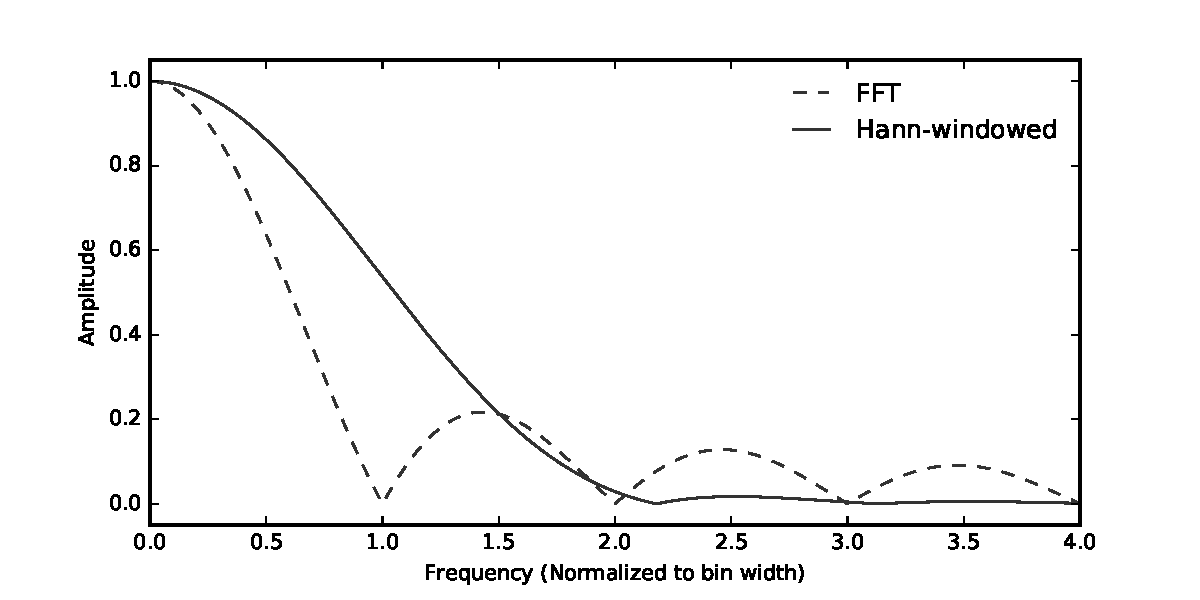
\includegraphics[width=\textwidth]{./figures/fft_resp}
 
 \caption{Amplitude response of the DFT, compared to amplitude response of a Hann-windowed DFT. \label{fig:fft_resp}}
\end{figure}

The DFT is computed over a finite number of samples, $N$, also known as the \emph{window length}. As the window length is not infinite, the response of the DFT is not perfect, resulting in spectral leakage (Fig.~\ref{fig:leakage}). This can be understood if we consider that the DFT
\begin{eqnarray}
X(k) & = & \sum_{n=0}^{N-1}x(n)e^{-2\pi ink/N} \\
     & = &  \sum_{n=-\infty}^{\infty} \Pi (n)x(n)e^{-2\pi ink/N}\\
     & = & \mathcal{F}\{\Pi(n)\}*X'(k)
\end{eqnarray}
where $\mathcal{F}$ denotes the Fourier transform, and $\Pi(n)$ the rectangle (or tophat) function:
\begin{equation}
\Pi(n) = \begin{cases}
	0 & \mbox{if } n < 0 \\
	1 & \mbox{if } 0 \leq n \leq N-1 \\
	0 & \mbox{if } n > N-1, \\
\end{cases}	
\end{equation}
which is Fourier paired with the sinc() function\footnote{This is the same relationship as that between light passing through a single slit aperture and its far-field diffraction pattern}. In other words, we can consider the finite length of the DFT as effectively convolving the perfect Fourier transform response $X'(k)$ with a sinc function. The undesirable peaks of the sinc function are referred to as \emph{sidelobes}.

\begin{figure}[t]
 \centering
 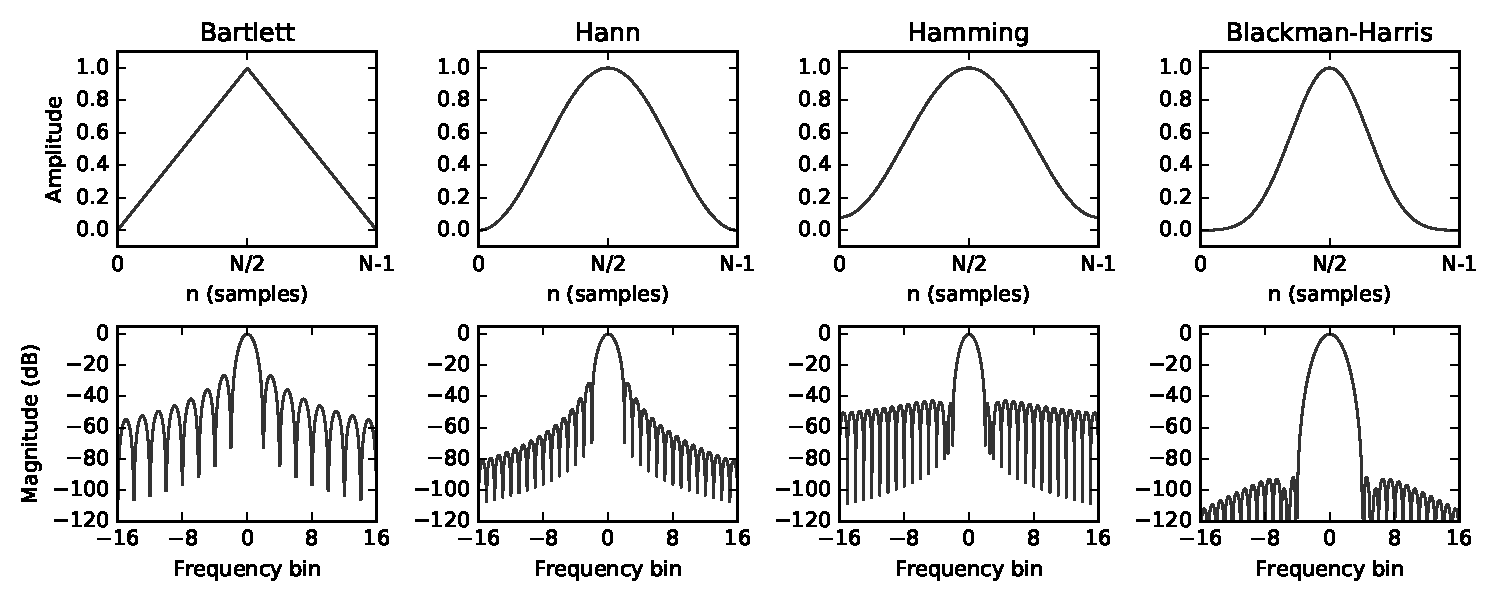
\includegraphics[width=\textwidth]{./figures/window_fns}
 \caption{Four common windowing functions ($w(n)$, top) and their corresponding squared Fourier transforms ($|W(k)|^2$, bottom). Outside of the range [0, $N-1$], the function $w(n)=0$ for all windows. \label{fig:window_fns}}
\end{figure}

Windowing functions\citet{SvenGade1987} improve the response of a DFT, by somewhat mitigating sidelobe response, at the expense of increasing the channel width. They are applied by multiplying the signal $x(n)$ by a weighting function, $w(n)$:
\begin{eqnarray}
X_w(k) & = & \sum_{n=0}^{N-1}w(n)x(n)e^{-2\pi ink/N} \\
       & = & W(k)*X(k).
\end{eqnarray}
The take-home message of all this is that DFT channels have a non-zero response outside their passband (Fig.~\ref{fig:fft_resp}), and that applying a windowing function can improve their response. 

Windowing functions are also important in the design of digital filters (Sec.~\ref{sec:filters}). Some common windowing functions and their frequency-domain magnitude responses are shown in Fig.~\ref{fig:window_fns}; their functional forms are given in Tab.~\ref{tab:window_fns}. The most appropriate windowing function is dependent upon application; for digital spectrometers, the Hamming and Hann windows are commonly applied.

%A more dramatic improvement may be achieved by using an lowpass filter frontend before the DFT \citep{Bellanger:1976p7898}, to form what is known as a polyphase filterbank. This approach is detailed further Sec.~\ref{sub:pfb}. 

%Figure~\ref{fig:PFB-num-taps} compares the spectral response of a standard DFT (`vanilla'), Hamming windowed DFT, and polyphase filterbank, for a single channel. An example showing a 16-channel, 4-tap Hamming window-based polyphase filterbank is shown in Figure~\ref{fig:PFB-8tap-16ch-example}.

%A filterbank is simply a collection of filters, a simple example being a highpass and lowpass filter pair. I discuss here filterbanks where each filter has identical passband characteristics and evenly spaced central frequencies, such as the 16 channel filterbank shown in Figure~\ref{fig:PFB-8tap-16ch-example}. This equally spaced form is the most commonly implemented for radio astronomy applications. 



\begin{table}
	\caption{Some common windowing functions, used in digital filters and DFT filterbanks. Note that in this table, coefficients have been rounded to four significant digits. \label{tab:window_fns}}
	\begin{tabular}{l l }
	\hline
	Weighting function      & $w(n)$                        			\\
	\hline
	\hline
	Uniform  (rectangular)   &  1                           			\\
	Bartlett (triangular)    &  $1 - (|n| / (N-1)$               	\\
	\hline
	\emph{General form:}    & $a_0 - a_1~cos(\frac{2\pi n}{N-1})$ \\
	Hann                     & $a_0=0.50 \quad a_1 = 0.50$ 	\\
	Hamming             & $ a_0 = 0.54 \quad a_1 = 0.46$   	\\
	\hline
	
	 \emph{General form:} &$a_0 - a_1~cos(\frac{2\pi n}{N-1}) + a_2~cos(\frac{4\pi n}{N-1}) -
	 					   a_3~cos(\frac{6\pi n}{N-1}) $	 \\
	 Nutall          & $a_0=0.3558\quad a_1=0.4874\quad a_2=0.1442\quad a_3=0.0126$ \\
	 Blackman-Nutall & $a_0=0.3636\quad a_1=0.4892\quad a_2=0.1366\quad a_3=0.0106$ \\
	 Blackman-Harris & $a_0=0.3588\quad a_1=0.4883\quad a_2=0.1413\quad a_3=0.0117$ \\
	\hline
	\end{tabular}

\end{table}



\subsection{Finite impulse response filters}\label{sec:filters}

A finite impulse response (FIR) filter is the windowed moving average of an input sequence $x(t)$. An FIR filter computes the sum 
\begin{equation} 
y(t)=\sum_{k=0}^{K-1}h(k)x(t-k),\label{eq:FIR-filter}
\end{equation}
where $y(n)$ is the output sequence, and $h(k)$ is a set of $K$ coefficients used for weighting. The upper summation bound, \emph{K}, is called the number of taps.\emph{ }A streaming implementation of an FIR filter is shown in Figure~\ref{fig:fir}.

\begin{figure}
 \centering
 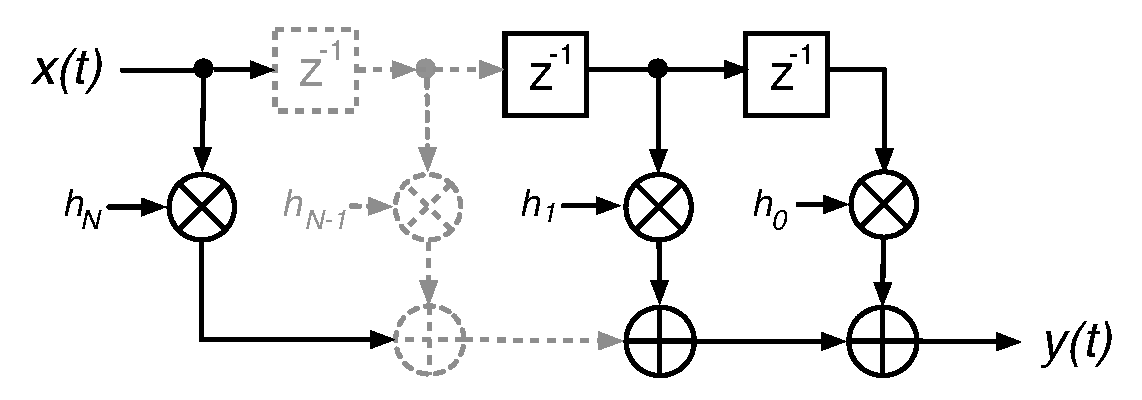
\includegraphics[width=0.8\textwidth]{./figures/fir_filter}
 
 \caption{N-tap FIR filter block diagram. An FIR filter applies a weighted sum to the input sequence $x(t)$, outputting the filtered signal $y(t)$. \label{fig:fir}}
\end{figure}

If we apply downsampling by $\downarrow D$ to an FIR filtered signal, we only keep the outputs $t=mD$, $m\in\mathbb{Z}^{+}$. A $\downarrow D$ downsampled filter will alias spectra centered at any multiple of the output sample rate to baseband. In such cases it is more efficient to only compute the terms we wish to keep: 
\begin{equation}
y(mD)=\sum_{k=0}^{K-1}h(k)x(mD-k).\label{eq:FIR-filter-decimated}
\end{equation}
One way we can accomplish this is to use a polyphase decimating filter, which is discussed below. 



\subsection{Polyphase FIR filters}

A common DSP technique is to decompose an input sequence $x(t)$ into a set
%\begin{equation}
%\mathbb{P}=\begin{Bmatrix}x_{k}(t) & k\in(0,P-1)\end{Bmatrix}
%\end{equation}
of $P$ sub-sequences, $x_{k}(t)$, each of which is given by 
\begin{equation}
x_{k}(t)=(\downarrow P)(z^{-k})x(t).
\end{equation}
This is known as polyphase decomposition. As a simple example, even and odd decomposition of the signal $x(t)$ is achieved when $P=\mbox{2}$:
\begin{eqnarray}
x_{0}(t) & = & \left\{ x(0),x(2),x(4),...\right\} \\
x_{1}(t) & = & \left\{ x(1),x(3),x(5),...\right\} .
\end{eqnarray}
More generally, an input stream may be decomposed into $P$ different `phases'.

\begin{figure}
 \centering
 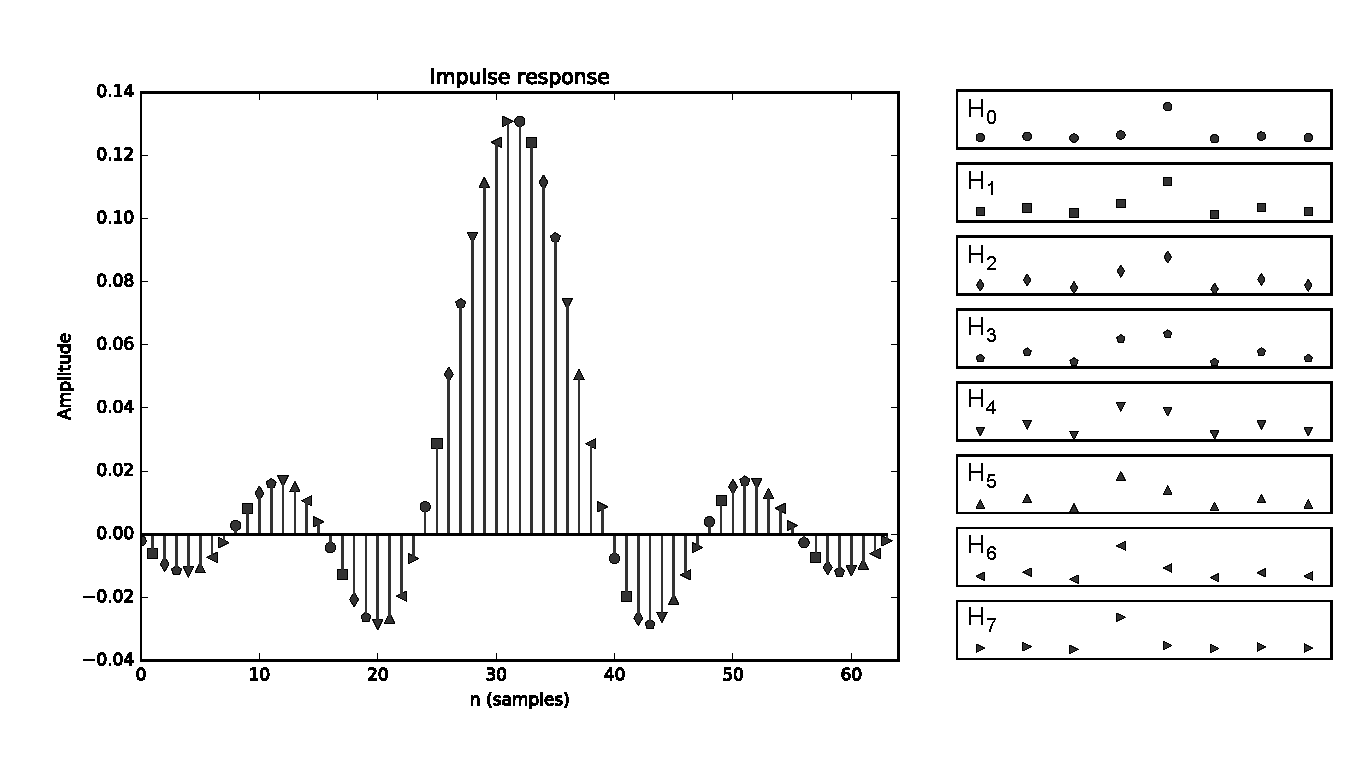
\includegraphics[width=\textwidth]{./figures/pfb_taps}
 \label{fig:pfb_taps}
 \caption{Example illustrating the polyphase decomposition of the coefficients h(k) of a 64-tap FIR filter (left) into 8 sub-filters (right). Each sub-filter has 8 taps; that is, P=8 and M=8.} %These sub-filters are re-combined in a decimating polyphase filter structure to form a filter with an impulse response equal to the original FIR filter (left).}
\end{figure}

Polyphase filter structures are often more efficient than standard finite impulse response filters when used in sample rate conversion. A $\downarrow P$ decimating FIR filter of length $K=MP$ can be constructed from $P$ discrete FIR filter `branches', each acting upon a different phase; that is
\begin{equation}
y(t)=\sum_{p=0}^{P-1}\sum_{m=0}^{M-1}h_{p}(m)x_{p}(t-m),\label{eq:FIR-polyphase-filter}
\end{equation}
This is known as a decimating polyphase filter. 

%For example, a $P=\mbox{4}$ branch polyphase filter with $M=\mbox{7}$ taps per sub-filter would compute the sum
%\begin{eqnarray}
%y(t) & = & \sum_{m=0}^{7}h_{0}(m)x_{0}(t-m)+\sum_{m=0}^{7}h_{1}(m)x_{1}(t-m)\nonumber \\
% & + & \sum_{m=0}^{7}h_{2}(m)x_{2}(t-m)+\sum_{m=0}^{7}h_{3}(m)x_{3}(t-m),
%\end{eqnarray}
%and has an output equivalent to a $\mbox{4}\times\mbox{7}=\mbox{28}$ tap standard FIR filter with 4:1 downsampling. 

Decimating polyphase filter structures are more efficient than standard FIR filter based downsampling techniques. If $\downarrow D$ downsampling occurs after the moving average of Equation~\ref{eq:FIR-filter}, we compute \emph{D} sums, but keep only 1 in \emph{D} of these. This is inefficient. In comparison, Equation~\ref{eq:FIR-polyphase-filter} only computes the output values that are of interest. 
%A comparison of two decimating filters is shown in Figure~\ref{fig:polyphase-filters}. Figure~\ref{fig:polyphase-filterb} is a polyphase type structure, but decimation occurs after summation. Conversely, Figure~\ref{fig:polyphase-filterb} shows a more efficient implentation where decimation occurs before summation. By the noble identities (see \citep{Vaidyanathan:1990p6127}), the output of this second filter is identical to that in Figure~\ref{fig:polyphase-filterb}.
Further discussion of polyphase filters is given by Vaidyanathan\citet{Vaidyanathan:1990p6127}.

\subsection{The Fast Fourier Transform\label{sub:fft}}

The Fast Fourier Transform\cite{Cooley1965, BookBrighamFFT} (FFT) is a highly efficient algorithm for computing the DFT of a signal with regularly-spaced samples\footnote{Nyquist and quadrature sampled signals have regularly spaced samples.}. To directly compute the DFT
\begin{equation}
X(k)=\sum_{n=0}^{N-1}x(n)e^{-2\pi ink/N}\label{eq:dft1}
\end{equation}
would require of order $O(N^2)$ operations, but the FFT algorithm reduces this to only $O(N \rm{log_2}$$N)$ operations. FFT implementations generally exhibit best performance when $N$ is a power of 2. 

For real-valued data, only $N/2$ channels are unique. FFT algorithms often exploit this for increased efficiency, by recasting the real-valued input data as complex values.

\section{Digital spectrometers}
As discussed in Sec.~\ref{sec:intro}, there are two equivalent paths that may be used to compute the PSD of a signal, as shown in  Fig.~\ref{fig:wiener}, referred to as ACS and FTF systems. As the DFT must be computed over a finite number of points, ACS and FTF systems have different characteristics. 

The first digital spectrometer used for radio astronomy was developed by Weinreb\citet{Weinreb:1963p10042} in 1963 -- two years before the FFT algorithm was introduced by Cooley \& Tukey\cite{Cooley1965}. This 1-bit ACS was used to observe the 18-cm wavelength hydroxyl (OH) absorption line in the spectrum of Cassiopeia A, providing the first evidence of OH in the interstellar medium \citep{Weinreb:1963p9992}. The first reference to FTF spectrometers for radio astronomy can be found in Chikada et. al.\citet{Chikada:1987p10044}; however FTF spectrometers did not enjoy widespread adoption until much later. The PFB architecture was first introduced by Schafer\cite{Schafer1973} in 1973 and expounded by Bellanger\cite{Bellanger:1976p7898} in 1976, but was not introduced for the purposes of radio astronomy spectrometry until 1992\cite{Duluk1992}. Bunton\cite{Bunton2000} further popularized the PFB within radio astronomy in 2000, suggesting its use in radio interferometer correlator systems. Given their growing ubiquity, PFB systems (which are essentially enhanced FTF spectrometers) are detailed at length in Sec.~\ref{sub:pfb}.

\subsection{Autocorrelation spectrometers}\label{sub:acs}

Digital autocorrelators implement delay-and-multiply circuitry using digital delays -- shift registers -- and digital multiplier cores to compute signal products. For an ACS implementation, the PSD (Eq.~\ref{eq:psd}) is computed for only a discrete range of delays, $\tau$. The spacing of lags in an ACS determines how much bandwidth it can process without aliasing occurring. The Nyquist criterion requires two taps per wave period at the highest frequency (shortest wavelength) signal of interest.

ACS systems exhibit poorer spectral leakage than FTF systems, due to the order of operations in Fig.~\ref{fig:wiener}. They also require more compute operations, $O(N^2)$, than FTF implementations, which require only $O(N~log_{2}N)$ operations. With current digital technology there is no compelling reason to implement an ACS spectrometer. The prevalence of ACS systems in early digital spectrometers may be explained by two reasons: for 1-bit data they can be implemented using boolean circuits, and they pre-date the FFT algorithm. 

\subsection{Fourier transform spectrometers}\label{sub:ftf}

FTF spectrometers compute the PSD of a signal by applying a DFT of length $N$ to an input signal, squaring the DFT output, then taking an average over time. 

%It is important to note that the DFT is computed over windows of length $N$ on the signal $x(t)$, which is essentially infinite in length. 
For a signal with sampling rate $\nu_s=2B$, each DFT channel has a bandwidth $B/N$, and a quadrature-sampled output rate of $\nu_s/2N = B/N$. As mentioned in Sec.~\ref{sub:sampling}, the DFT (Eq.~\ref{eq:dft1}) may be thought of as the mixing of the input signal with a bank of oscillators, followed by an averaging with a square window function. In effect, this is a simple filterbank. 
%Thinking of the DFT as a filterbank, instead of as a transformation of a time-domain signal into a frequency-domain signal, gives an alternative insight into how a spectrometer works.

%For real-sampled data the negative frequencies contain no extra information, so they need not be computed. This leaves a a bank of $N/\mbox{2}$ filters, evenly spaced over a bandwidth $\nu_{s}/\mbox{2}$. 

In general, computing Eq.~\ref{eq:dft1} for each value of $\nu_0$ requires $N$ multiplications, and $N$ additions. Since $\nu_0$ can take $N$ independent values itself, the total cost of implementing a DFT filterbank is $N^2$ operations per transform. If one transform is computed for every $N$ samples digitized, then the computation rate is of order $\nu_sN$ operations each second. 

The FFT (Sec.~\ref{sub:fft}) allows Eq.~\ref{eq:dft1} to be evaluated in $O(N\log_2N)$ operations, or $\nu_s\log_2N$ when performed every $N$ samples. With computational savings of order $N / \log2{N}$ the FFT is an extraordinarily powerful algorithm, which is used heavily throughout radio astronomy. For a spectrometer of $~10^4$ channels, the FFT algorithm requires approximately $0.1\%$ as many operations as an ACS system.


\subsection{Polyphase filterbanks}\label{sub:pfb}

A PFB is a computationally efficient implementation of a filterbank, constructed from an FFT preceded by a prototype polyphase FIR filter frontend.\citet{Bellanger:1976p7898, Harris2011} PFB-based spectrometers offer vastly lowered spectral leakage over both ACS and FTF architectures. 
%For radio astronomy purposes, high interchannel isolation is important so that spectral features are not smeared out, and so the spectrometer is more resilient to the high levels of radio frequency interference (RFI) emitted from terrestrial sources. Polyphase filterbanks are therefore the best candidate for radio astronomy spectrometers, if computationally affordable.

The PFB exploits the fact that a lowpass filter with coefficients $h(k)$, can be converted into a quadrature bandpass filter with central frequency $\omega_{k}=2\pi\nu$ by multiplying the coefficients by $e^{i\omega_{k}t}$ . That is, 
\begin{equation}
h_{bpf}(k)=h(k)e^{i\omega_{k}t}.\label{eq:lowpass-to-bandpass}
\end{equation}
Now, suppose we have implemented a decimating lowpass polyphase filter. The output of each branch is 
\begin{equation}
y_{p}(t)=\sum_{m=0}^{M-1}h_{p}(m)x_{p}(t-m),
\end{equation}
where $h_{p}(m)$ are coefficients from our prototype lowpass filter. If we follow this by a DFT, as in Fig.~\ref{fig:pfb_fir_fft}, we then have 
\begin{eqnarray}
Y(k) & = & \sum_{p=0}^{P-1}y_{p}(t)e^{-2\pi ikp/P}\\
 & = & \sum_{p=0}^{P-1}\sum_{m=0}^{M-1}h_{p}(m)e^{-2\pi ikp/P}x_{p}(t-m).
\end{eqnarray}
Comparing this form to Equation~\ref{eq:FIR-filter-decimated} and Equation~\ref{eq:lowpass-to-bandpass}, we recognise that the output
of this structure is equivalent to a set of $\downarrow P$ decimating polyphase filters,
%\begin{equation}
%\mathbb{F}=\begin{Bmatrix}h_{k}(m), & k\in(0,P-1)\end{Bmatrix}
%\end{equation}
where the central frequency of each filter is shifted by an amount $\mbox{2}\pi ik/P$. 
%For data sampled at the Nyquist rate $\nu_{s}$, this filterbank consists of $N$ filters spanning $-\nu_{s}/\mbox{2}$ to $\nu_{s}/\mbox{2}$, with each filter separated by $\nu_{s}/\mbox{2}N$.

\begin{figure}
 \centering
 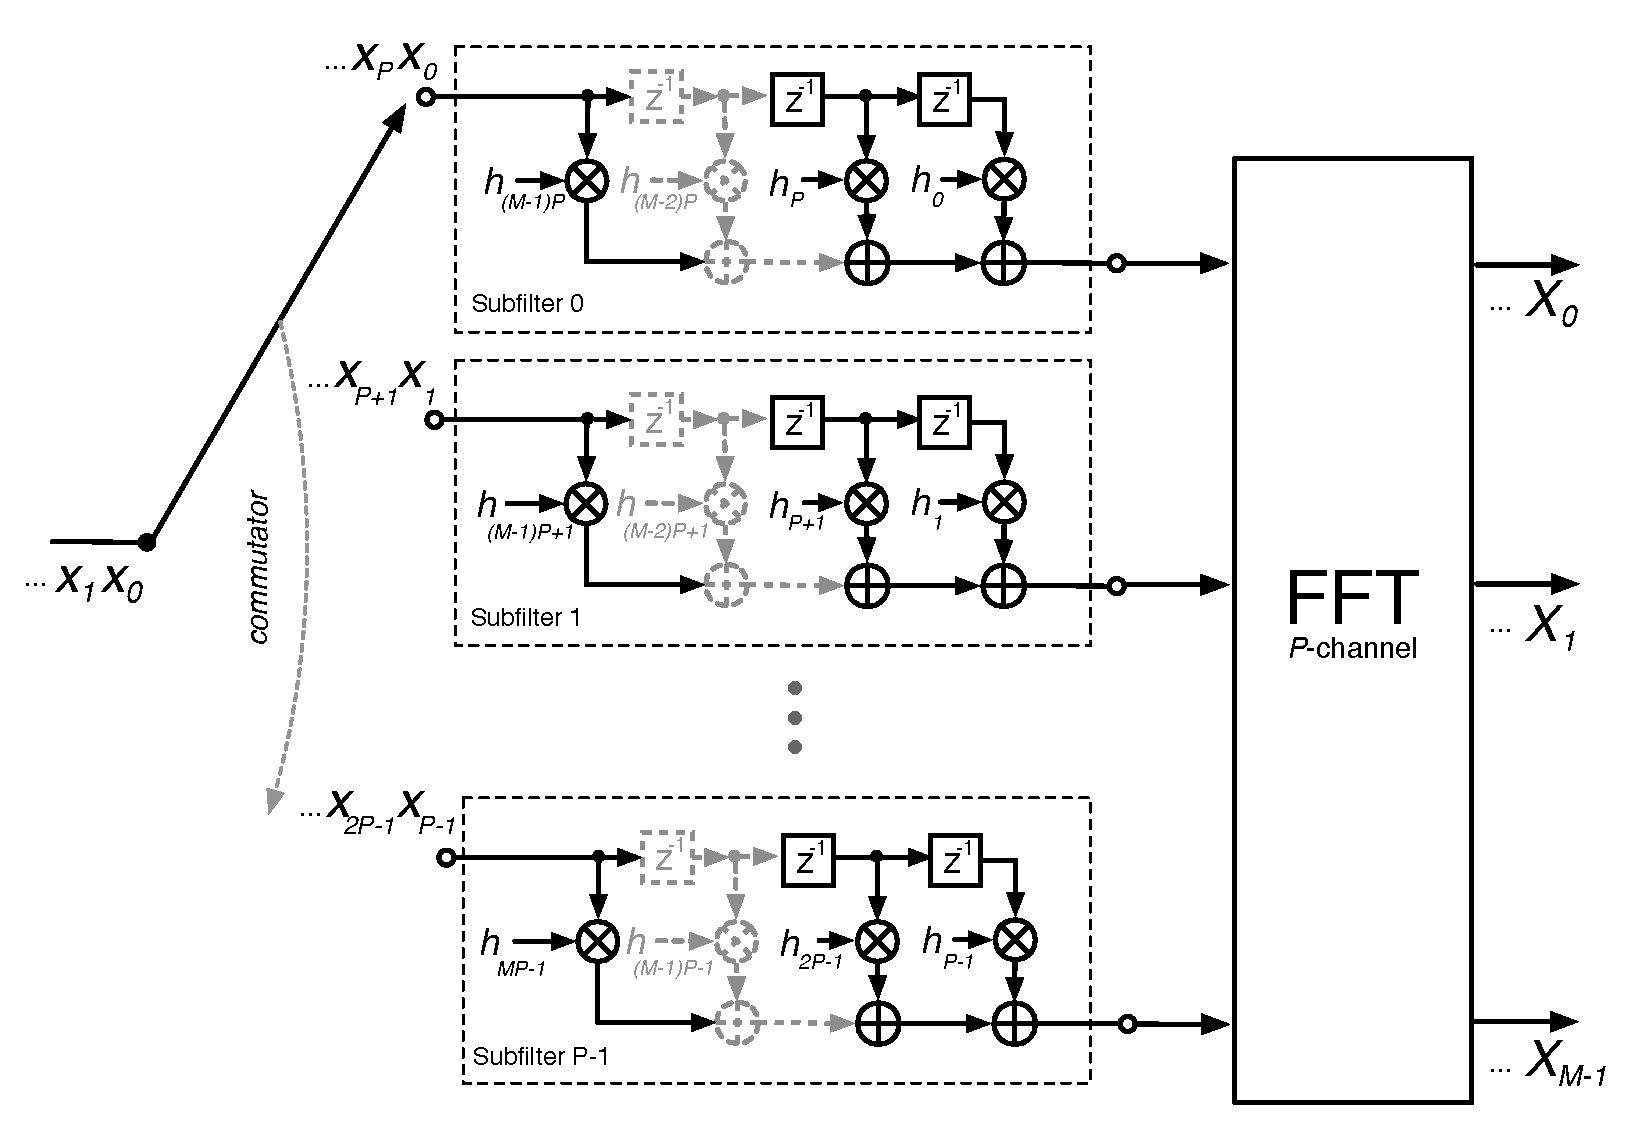
\includegraphics[width=\textwidth]{./figures/pfb_fir_fft}
 \caption{Polyphase filterbank streaming implementation. A PFB is formed when a polyphase FIR filter structure is combined with a DFT.\label{fig:pfb_fir_fft}}
\end{figure}

\begin{figure}
 \centering
 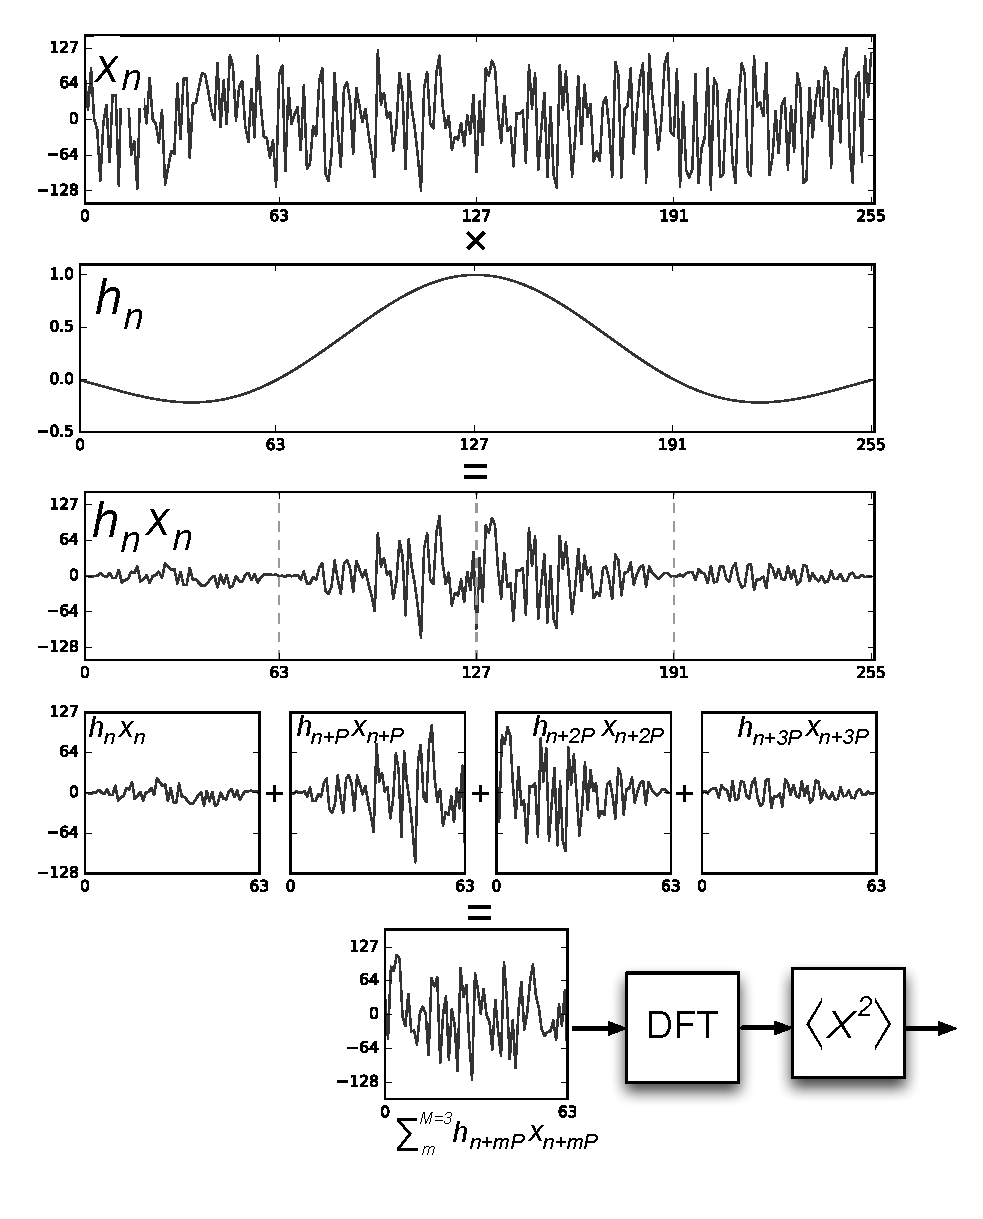
\includegraphics[width=\textwidth]{./figures/pfb_chart}
 \caption{Graphic representation of a PFB spectrometer, illustrating the action of the polyphase FIR filter frontend.\label{fig:pfb_chart}}
\end{figure}


%\subsubsection{Overlapping filterbanks}

%\subsection{Implementation comparison}\label{sub:comparison}

%ACS and FTF architectures differ in both their spectral response and the number of computations required to implement them. For regularly sampled data, the Fast Fourier Transform (FFT) algorithm may be used to compute the DFT (see, for example, \citep{BookBrighamFFT}), which reduces the number of computations required from $O(N^{2})$ for to $O(Nlog(N))$. In Chapter~4 of \citep{Taylor1999}, Romney shows that the ratio of multiplies for the two architectures is 
%\begin{equation}
%R_{\frac{ACS}{FTF}}=\frac{n_{t}}{\mbox{2}log_{2}(n_{t})},
%\end{equation}
%where $n_{t}$ is the number of samples per FFT or lag correlation. So in general, FTF architectures require fewer computations than their equivalent ACS counterpart. Romney also shows that the spectral response of FTF and ACS architectures differ, with ACS architectures having a $sinc$ reponse, and FTF architectures posessing a $sinc^{2}$ response. The result is that interchannel isolation is better in FTF architectures (first sidelobe at $\sim-\mbox{13.6}$ dB), than in ACS architectures ($\sim-\mbox{6.8}$ dB). 

\subsection{Zoom modes}

The output of each channel of a DFT-based filterbank is a critically-sampled quadrature time stream of its own right (before the signal is squared, that is). Higher spectral resolution can be achieved by passing the output of a `coarse' first-stage filterbank channel into a secondary DFT to apply finer channelization, after which the samples may be squared and averaged to compute the PSD. Spectrometers that employ this approach are known as \emph{zoom spectrometers}. 

An extension of the zoom spectrometer can be used to efficiently develop filterbanks of many millions of channels. The second-stage filterbank in a zoom spectrometer only needs to run at $1/N$ the rate of its first-stage filterbank. If the second-stage DFT (of length $M$) is run at the same speed as the first-stage filterbank, one can run the second-stage DFT on every first-stage channel, instead of just one. The result is a filterbank with $N\times M$ channels. 

To do so requires that the output of every first-stage channel is buffered so that there are $M$ samples per channel, then data must be rearranged and fed to the second-stage DFT in channel order. This reorder can be considered a matrix transpose (also called a \emph{cornerturn}), rearranging from ($N$, $M$) to ($M$, $N$) order.

As an example, a zoom-style spectrometer with $N$=$M$=1024 has $N\times M / 2$=524,288 channels total. 


\section{Alternative spectrometer implementations}

\subsection{Swept spectrometer}\label{swept-spectrometer}

%\begin{figure}
% \centering
% 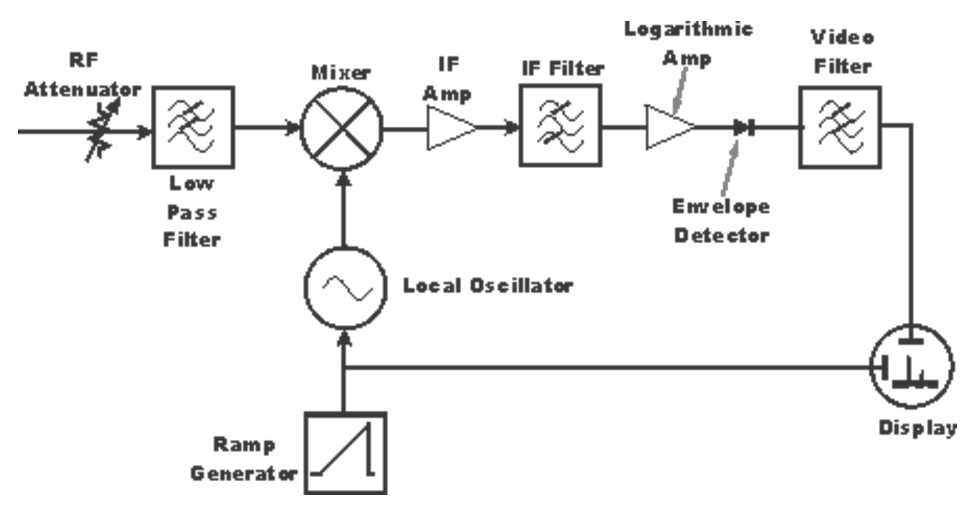
\includegraphics[width=\textwidth]{./figures/temp_spec_an_diagram}
% % analog-autocorr-crop.pdf: 0x0 pixel, 0dpi, nanxnan cm, bb=
% \label{fig:swept-an}
% \caption{Swept spectrum analyzer block diagram, need to remake. We can't use this image because a) it's low quality and b) it's not ours. \label{fig:swept}}
%\end{figure}

A \emph{swept spectrometer} uses a variable oscillator with a heterodyne
circuit and a low pass filter. The oscillator is typically varied, i.e.~swept, through a range of desired frequencies. As it is swept through the desired frequency range, the power of the low pass filter's output is measured and recorded. Most analog spectrum analyzers operate in this manner.

An advantage of swept spectrometers is that they can operate over large RF bandwidths. However, as only a fraction of the band is detected at any one time, less integration time is available per frequency channel. 
%For a swept spectrometer with $N$ channels with a sweep time of $t_{\rm{sweep}}$, the integration time available per channel is $t_{\rm{sweep}}/N$. It follows that  
The RMS noise per channel in a swept spectrometer is $\sqrt{N}$ higher than an equivalent FTF spectrometer covering the entire RF bandwidth. As such, swept spectrometers are best suited for cases where signals of interest are strong and wideband. 

\subsection{Analog filterbank}\label{analog-filter-bank}

An analog filterbank is just what its name implies: a bank (or collection) of analog filters. The analog filters are designed to pass through different ranges of frequencies. The power of each filter's output is measured and recorded, from which spectral features can be discerned. 

% By creating a bank of filters with adjacent and non-overlapping passband frequencies one can get a complete picture of the input signal's spectrum.

Analog filterbanks may offer very wide bandwidths, but design of very narrowband filters is challenging. Additionally, the input signal must be split multiple times, and each time the signal is split, its power halves. Unlike digital systems, the shape and gain of each filter may differ. For these reasons, analog filterbanks are uncommon in modern radio astronomy.

\subsection{Analog autocorrelator spectrometers}\label{sub:analog-acs}
%The power spectrum of a signal, $S(f)$,  is related to the signal's autocorrelation function, $R(\tau)$, over a range of time lags, $\tau$, by Fourier transform:
%\begin{equation}
%\label{spec-from-autocorr}
% S(f) = \int_{-\infty}^{\infty} R(\tau)e^{-2\pi i \tau f} \,\mathrm{d}\tau \,.
%\end{equation}

%Thus, if one can build a device to measure the autocorrelation function of a signal of interest, it is straightforward to obtain the signal's power spectrum.
%When integrated over a time $T$, the autocorrelation of a signal specified by the time-varying voltage $v(t)$ is defined by 

%\begin{equation}
%\label{autocorr}
% R(\tau) = \frac{1}{2T} \int_{-T}^{T} v(t)v(t+\tau) \,\mathrm{d}t \,.
%\end{equation}

%Since $v(t)$ is a real-valued function $R(\tau)$ is necessarily symmetric about positive and negative lags, so only one half need be measured. Furthermore, the symmetry of $R(\tau)$ means that the only contributions to $S(f)$ are from the even parts of the complex exponential in Equation \ref{spec-from-autocorr}. The computation of the power spectrum can then be reduced to:

%\begin{equation}
%\label{spec-from-autocorr-reduced}
% S(f) = 2\int_{0}^{\infty} R(\tau)\cos{(2\pi \tau f)} \,\mathrm{d}\tau \,.
%\end{equation}


An analog ACS uses analog circuitry to implement multipliers and propagation times through carefully constructed delay lines to implement the desired tap delays. 
%A typical schematic of an analog ACS is shown in Fig.~\ref{fig:analog-autocorr}. Here, outputs of each correlator tap are digitized after a small amount of time-averaging. Further averaging can take place digitally before computation of the power spectrum via cosine transform. 
Details of specific scientific deployments of analog autocorrelation spectrometers can be found in \cite{Erickson2007} and \cite{Harris1998}.

The main advantage of the analog autocorrelator over its digital counterpart (Sec.~\ref{sub:acs}) is that digitization need only take place at a rate commensurate with the averaging period of the correlator, rather than the bandwidth of the input signals. For this reason, analog ACS spectrometers are usually seen in systems that have instantaneous bandwidths of many gigahertz. Their major disadvantage is that the number of physical components required scales with the number of channels, making analog ACS systems with many channels --- readily implemented by digital systems ---  infeasible.


%\begin{figure}
% \centering
% 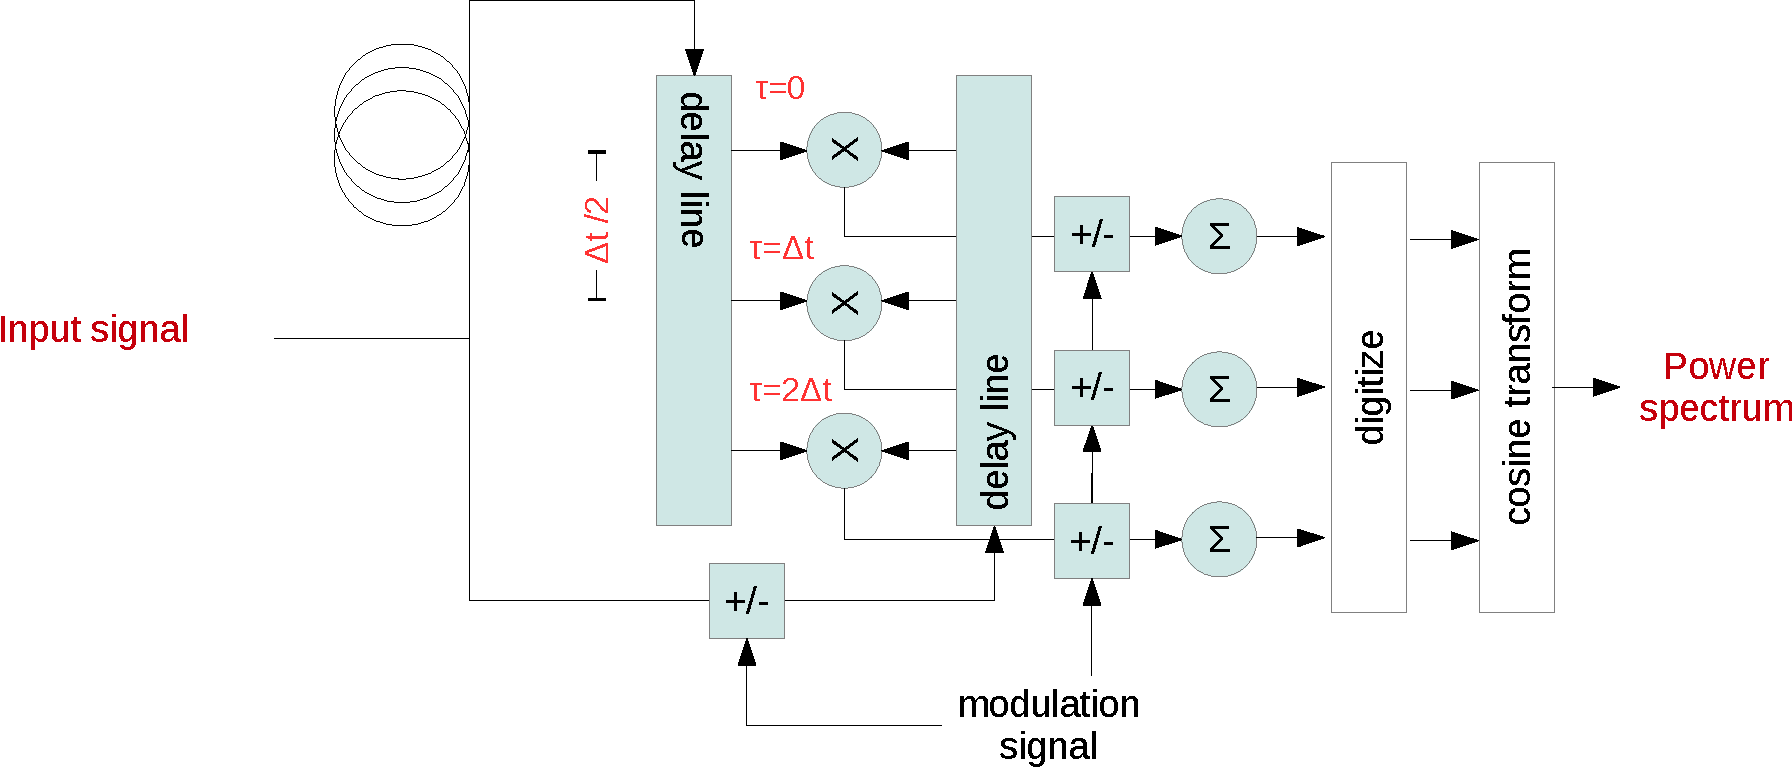
\includegraphics[width=\textwidth]{./figures/analog-autocorr-crop.pdf}
% % analog-autocorr-crop.pdf: 0x0 pixel, 0dpi, nanxnan cm, bb=
% \label{fig:analog-autocorr}
% \caption{An example implementation of an analog ACS. The input signal is circulated in opposite directions down a pair of delay lines. The signal is tapped on each delay line at points separated by propagation delays of $\frac{\Delta t}{2}$. Each tap computes an element of the correlation with lag $\tau=n\Delta t$.}
%\end{figure}

%Figure \ref{fig:analog-autocorr} also indicates circuitry for modulating the input and outputs of the correlator. Such switching can serve multiple purposes. Firstly, it is sometimes advantageous for cost or performance reasons to prefer square-law diode detectors in favour of multiplication circuitry. These have a respose to inputs $v_1$ and $v_2$ of
%\begin{equation}
% v_1^2 + v_2^2 + 2v_1v_2 \, .
%\end{equation}

%The last term is equal to the output of a multiplier, while the first two terms represent unwanted parts of the diode response. These unwanted terms can be eliminated by periodically alternating the sign of one of the inputs $v_1$ or $v_2$. This has no effect on the unwanted terms, but causes the last term to alternate sign. If, prior to time averaging, the sign of the diode output is flipped synchronously with the input then the unwanted terms will, up to a noise contribution, be removed.

%In general, the principal of modulating the desired part of a signal and then synchronously demodulating to cancel out unwanted contributions can be used to surpress a variety of unwanted effects in radio receivers, such as gain variation and cross-coupling. An operating telescope may have multiple such switching systems operating concurrantly at different frequencies targetting different effects. See, for example, \cite{Erickson2007}. 

%\subsection{Acousto-Optic}\label{acousto-optic}

%\subsection{Hybrid Analog-Digital}\label{hybrid-analog-digital}


\section{Current technology}

Most modern implementations of spectrometers in radio astronomy are PFB based, and use commercially available high-speed ADCs. Over the years, ADC input bandwidth has grown from kilohertz to the gigahertz we see today. Specifications of some example high-speed ADCs that are currently available are given in Tab.~\ref{tab:adcs}. 

\begin{table}
\begin{center}
\begin{threeparttable}
	\caption{Some example high-speed ADCs (i.e. wide input bandwidth) that are currently commercially available. \label{tab:adcs}}
	\begin{tabular}{c c c c c}
	\hline
	Sample rate & Input bandwidth & $n_{\rm{bits}}$ & Manufacturer & Part  \\
	(GS/s) & (GHz) & & & \\
    \hline
    5 & 2 & 8 & e2v & EV8AQ160 \\
	15 & 20 & 4 & Adsantec & ASNT7122  \\
	26 & 20 & 3\tnote{$\dag$} & Analog Devices & HMCAD5831  \\
	30 & 20 & 6 & Micram & ADC30 \\
	\hline
	\end{tabular}
	
  \begin{tablenotes}
  %\item [1] the first note ...
  \item[$\dag$] Plus overrange bit
  %\item[a] \url{http://www.adsantec.com/304-asnt7122-kma.html}
  \end{tablenotes}

\end{threeparttable}
\end{center}
\end{table}

Once analog signals are digitally sampled, a variety of signal-processing platforms are available on which to implement the algorithms described earlier in this chapter:

\paragraph{Central Processing Units (CPUs),} of the type found in widely available laptop and desktop computers, are capable of processing only relatively small bandwidths, but are cheap and very easy to program. Though largely superceded in modern high-bandwidth systems, past examples of CPU-based spectrometers in astronomy include \cite{Montebugnoli1996} and UC Berkeley's distributed SETI@home project \citep{Anderson2002}.


\paragraph{Graphics Processing Units (GPUs)} are processors with thousands of arithmetic cores, capable of performing many trillions of operations every second.
%GPUs are available as ``graphics cards'': expansion cards that can be added to off-the-shelf computer systems.
GPU development is driven by the computer gaming industry, but over the last decade an increasing focus has been placed by GPU manufacturers on General-Purpose GPU (GPGPU) computing uses. GPUs have gained significant traction in spectrometers where large FFTs are required in order to achieve high spectral resolution\cite{Kondo2010}.


\paragraph{Field Programmable Gate Arrays (FPGAs)} are logic chips which incorporate many thousands of arithmetic cores in a fabric of programmable logic and interconnect. FPGAs excel at processing large data rates and provide low-level interfacing capabilities, allowing them to be directly connected to modern ADC chips. While an increasing number of off-the-shelf FPGA platforms are available, the needs of radio astronomers often motivate the design of custom boards. FPGAs are also relatively difficult to program, with specialist knowledge of their underlying hardware details neede to utilise them efficiently. FPGAs have smaller quantities of memory than CPU or GPU processors, and are often used for high data-rate, coarse-resolution spectrometers \citep{Stanko2005, Finger2012}.

\paragraph{Application Specific Integrated Circuits (ASICs)} are custom-designed chips, with underlying circuitry dedicated to performing the operations defined by the designer. The custom nature of an ASIC makes it the most power-efficient computing platform though this efficiency comes at the cost of large development time and effort.
With the increasing performance and power-efficiency of FPGAs and GPUs, ASIC development is not as prevalent in radio astronomy as it once was.
However, ASICs may still be desirable for space-based spectrometers, where power-efficiency is paramount (see, for example, \cite{hochman2014splash}).

\paragraph{Hybrid systems.} In many cases a spectrometer may be heterogeneous in nature, with different stages of processing performed on different hardware platforms.
Frequently, FPGAs are used to facilitate interfacing a high speed ADC chip with a network of CPU or GPU signal processing devices \citep{Siemion2011}. 
Spectrometers such as the \emph{VEGAS} spectrometer at the Robert C. Byrd Green Bank Telescope \citep{Prestage2015} also utilise FPGAs for ADC interfacing and coarse channelisation, before signals are further filtered to a fine frequency resolution using GPUs.


\subsection{Common Infrastructure Developement}
%The rapid increasing performance of signal processing hardware and the common requirements of different observatories mean that sharing the development of new processing platforms incorporating the latest processors can be very beneficial to the radio astronomy community.

CPU and GPU processing platforms are developed by commercial entities, motivated by the non-astronomy markets. However, leveraging the latest hardware requires uses to have access to flexible programming tools and software libraries. A number of open-source projects have emerged trying to serve this need.
The \textsc{GNURadio} project\footnote{\url{gnuradio.org}} provides a software environment for rapid development of CPU-based instruments for processing radio signals.
A number of radio astronomy projects have also developed generic software pipelines for streaming data between Ethernet networks, CPUs and GPUs (see for example \textsc{HASHPIPE}\footnote{\url{https://github.com/david-macmahon/hashpipe}} and \textsc{Bifrost}\footnote{\url{https://github.com/benbarsdell/bifrost}}).

FPGA platforms are expensive to design and manufacture. For this reason, radio-astronomy groups such as the Collaboration for Astronomy Signal Processing and Electronics Research (CASPER\footnote{\url{https://casper.berkeley.edu}}) have developed a variety of general-purpose FPGA-based platforms which can interface with a suite of connectorized ADC cards.
CASPER provide a variety of open-source software tools and libraries with the aim of simplifying FPGA programming and enabling straightforward upgrading of instruments when newer more capable hardware becomes available.

%\section{Conclusions}

%Polyphase filterbanks have attractive characteristics for radio astronomy applications. They offer excellent interchannel isolation and can be implemented using efficient FFT based structures. Field Programmable Gate Arrays are a viable platform on which to implement wide bandwidth polyphase filterbank spectrometers.

\section{Acknowledgements}

The authors thank members of the CASPER collaboration for sharing their extensive knowledge with the wider community; all figures have been made available by the CASPER collaboration under the CC-BY license\footnote{\url{http://creativecommons.org/licenses/by/4.0/legalcode}}. D. Price thanks J. Moran for thorough discussion and debate on the virtues of polyphase filterbanks, J. Bunton for clarifying the history of PFBs in radio astronomy, and D. Werthimer and A. Wolszczan for providing the opportunity and motivation to develop this chapter. 

\bibliographystyle{ws-rv-van}
\bibliography{spectrometers,references}

\end{document}
